\section{Introduction}

As the availability of genetic data has increased,
so has our ability to infer evolutionary processes at finer scales.
An essential tool for evolutionary inference has been simulations,
and many flexible and efficient evolutionary simulators have been developed over the past decade \citep{hudson_testing_1983, hudson_test_1987, carvajal-rodriguez_simulation_2008, ohta_simulation_1974, hoban_computer_2012, bulmer_effect_1976}.
Until recently, little had been done to integrate different tools and to ensure compatibility of inferred models across studies.

A unifying thread that has emerged is the tree sequence data structure \citep{kelleher_efficient_2016}.
The tree sequence provides a way of concisely representing correlated genealogies along chromosomes.
Both msprime, an efficient coalescent simulator, and SLiM, the most widely used forward-in-time simulator,
record the genealogical history of all samples in a population in the form of tree sequences \citep{kelleher_efficient_2018, haller_tree-sequence_2019, haller_slim_2019}.
One of the major advantages of doing so in forward-in-time simulations is that it allows neutral mutations to be omitted.
By definition, such mutations do not impact the underlying genealogies, but they pose immense computational demand (due to bookkeeping).
Therefore, by omitting the neutral mutations from the forward step, it is possible to decrease computational resources dramatically.
After completion of the forward simulation, it is possible to simply overlay the genealogies with the neutral mutations if necessary.

As inference becomes ever more complex, now enabled by powerful simulation tools,
the need for easy and error-free dissemination of estimated models has increased.
Many researchers used to re-implement models independently,
a process which is error-prone and results in duplication of effort.
Indeed, a recent study described errors in the implementation of a demographic model in two published papers,
which affected the interpretation of biological signals \citep{ragsdale_lessons_2020}.

Stdpopsim is a community-driven open source developed to minimize these issues \citep{adrion_community-maintained_2020, lauterbur_expanding_2023}.
We organized a well-documented library with published simulation models from a range of organisms,
which can be accessed with simple Python and command-line interfaces.
The library contains demographic models, recombination maps and mutation rates for tens of species.
All the models have to pass a quality control method, in which an independent party validates the model independently.
Further, we provide a Python API to easily run simulations using the catalog, with msprime and SLiM as simulators on the backend,
decreasing even further the barrier to reproducing simulations.

In this chapter, I will present two vignettes of my contributions to the ecosystem of evolutionary simulation tools.
First, I describe a way to break up simulations of multiple populations, which was enabled by tree sequence recording.
Second, I describe the inclusion of selection models to stdpopsim,
and I illustrate the utility of stdpopsim by studying the power to detect sweeps along chromosomes.


\section{A way to parallelize multi-population simulations with tree sequences}

A major problem in simulation-based inference is the computational cost of simulations.
In many cases, it is possible to minimize the time cost of simulations by running them in parallel,
that is to divide up the simulation over many processes that can be executed concurrently over many CPUs (or cores).
It is not always clear how to divide a simulation into sub-tasks, however.

In the case of evolutionary simulations, a natural way to break up a big simulation might be population splits.
After a population splits into two (or more) subpopulations,
their histories become independent (assuming no migration).
Therefore, it is possible to parallelize a multi-population simulation by dividing the simulation over population splits.
The history of populations A, B and C (shown in \lcref{fig:pop_hist}) can be parallelized:
any two branches stemming from the same node are independent.

\begin{figure}[htp]
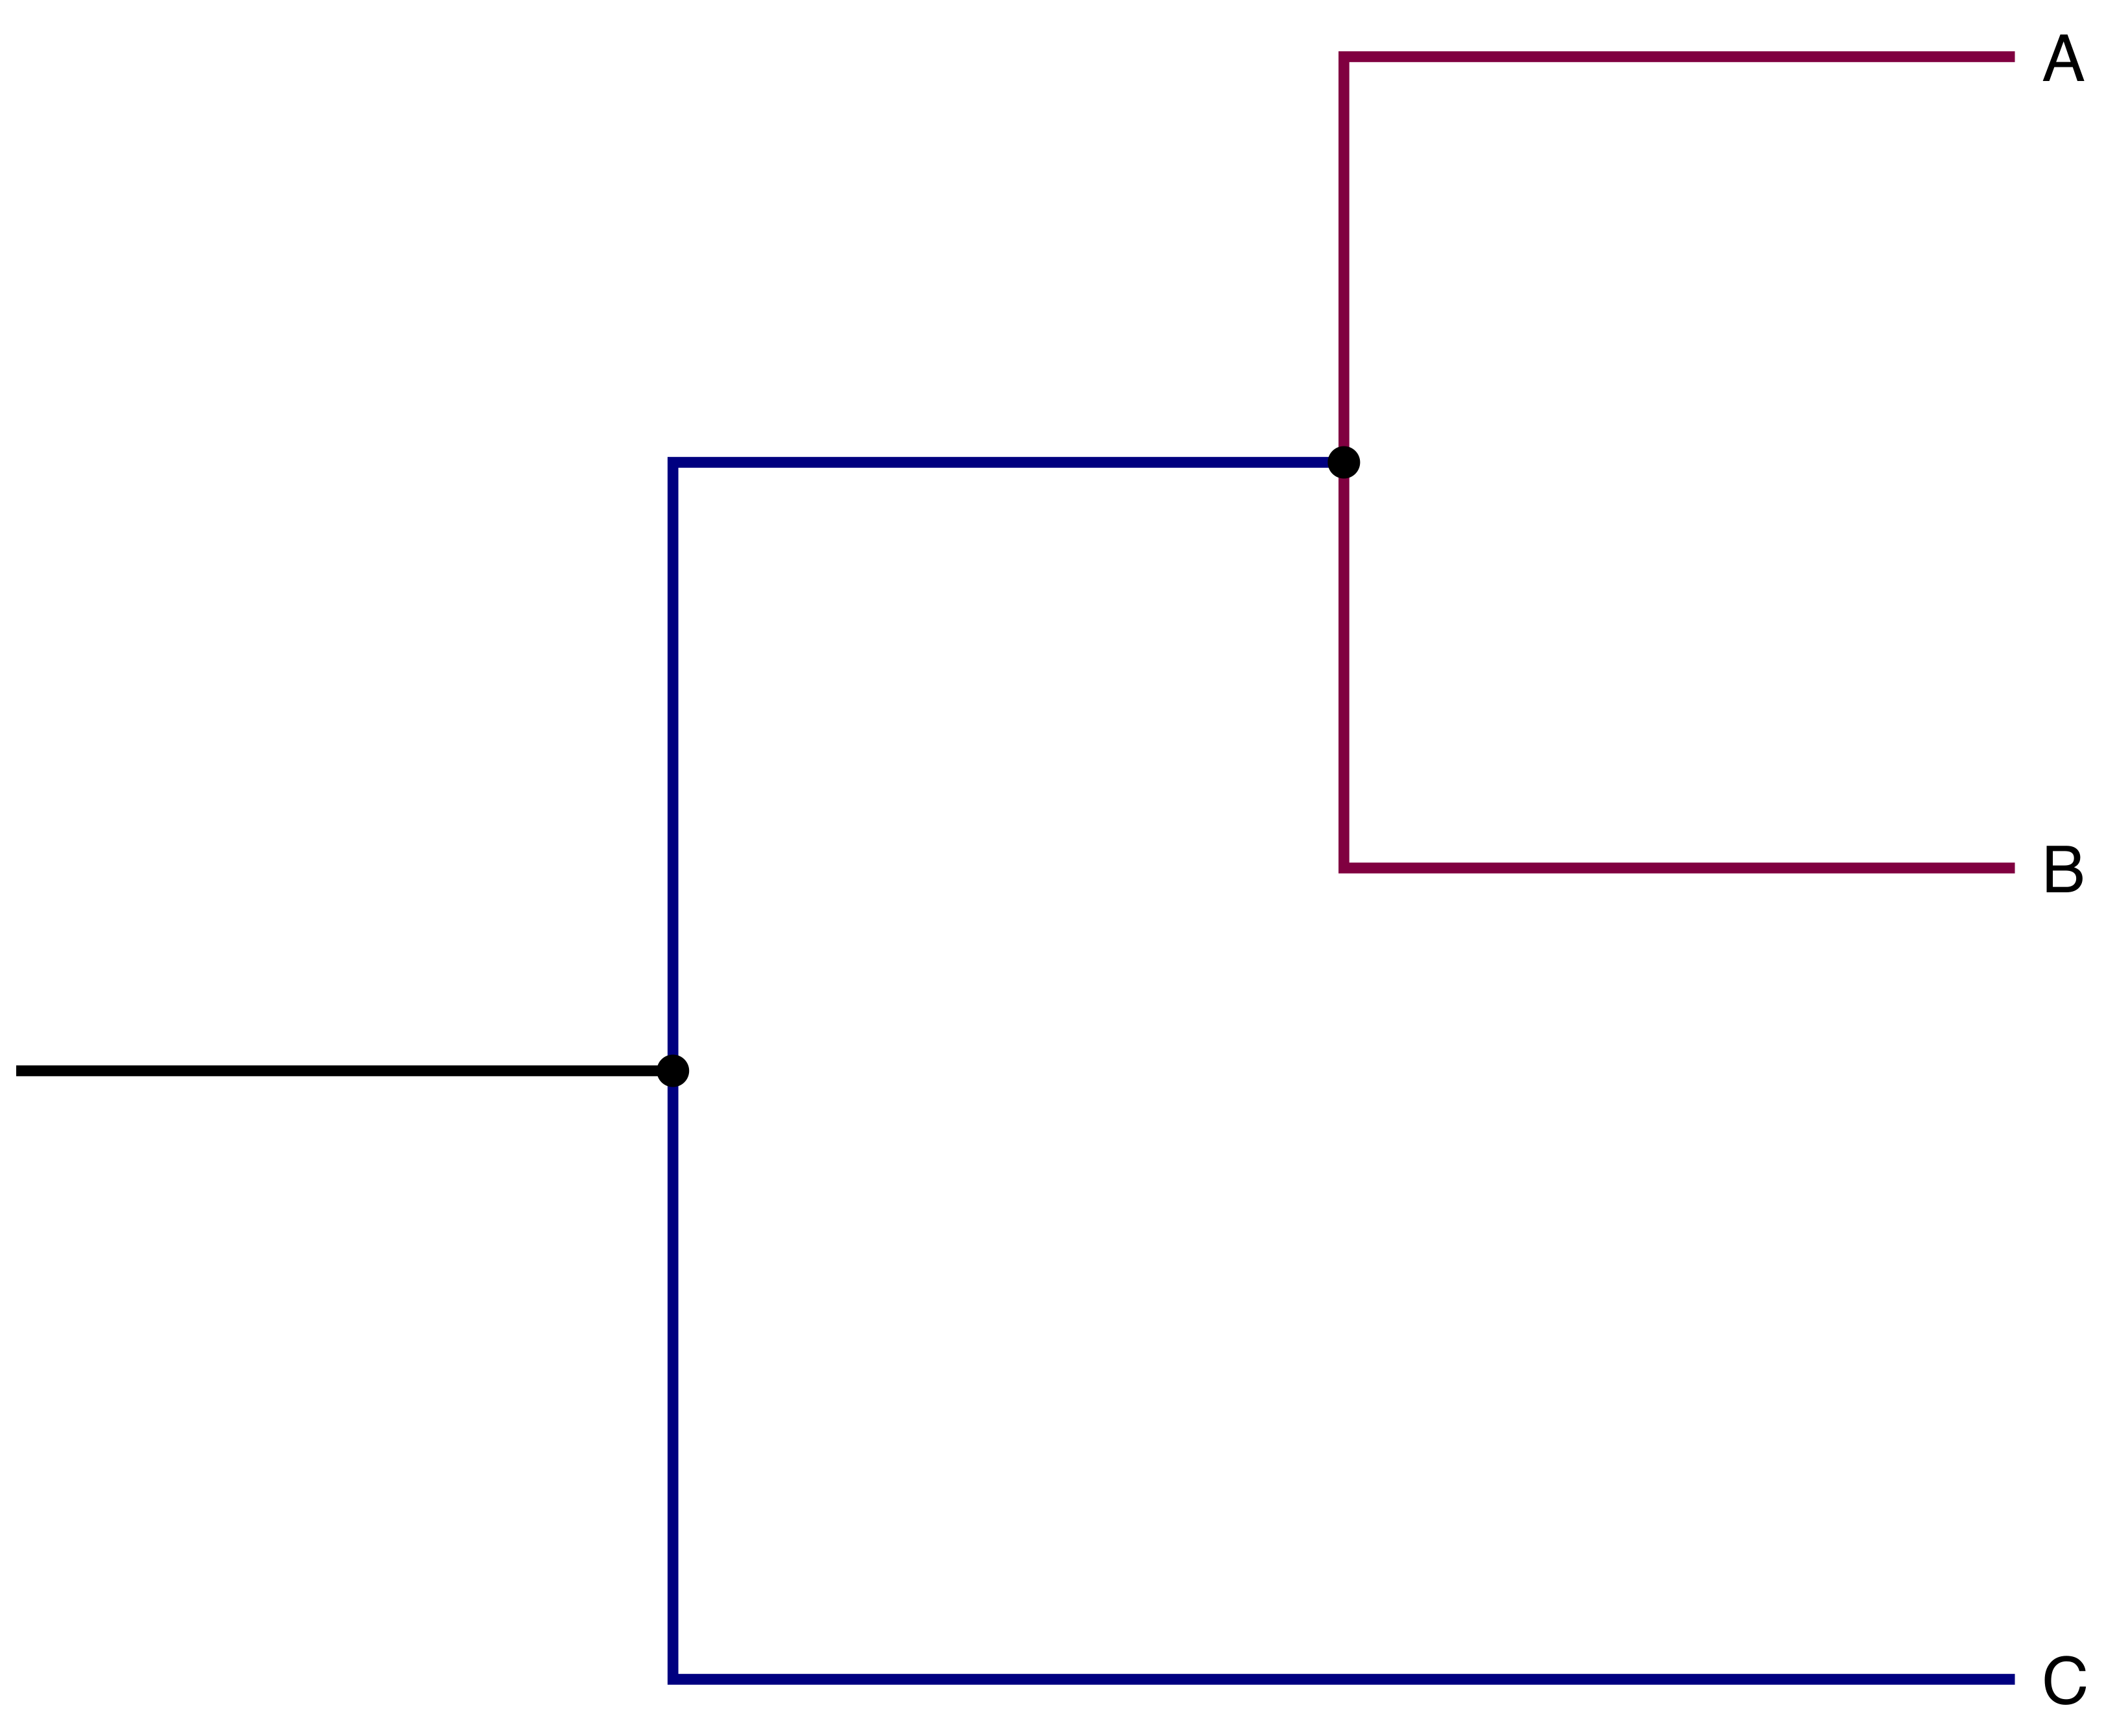
\includegraphics[width=0.5\linewidth]{{figures/phylo.png}}
\centering
\caption[Example of a population history]{
The relationships between populations A, B and C are depicted.
Note how branches of the same color can be simulated in parallel if there is no migration.
}
\label{fig:pop_hist}
\end{figure}

To parallelize the simulations, we need to
(i) simulate each branch of the tree independently and
(ii) put together the bits that are simulated independently at the end.
There are many ways to parallelize the simulations, but see \citet{rodrigues_vignette_2021} for an idea.
Below, I will describe the operation for putting together two (or more) tree sequences,
which has been implemented in \tskit (see \url{https://tskit.dev/tskit/docs/stable/python-api.html#tskit.TreeSequence.union} for the documentation).

The information underlying a tree sequence is stored as a collection of tables which define different features.
This simple tabular format allows for rapid accessing of information.
The main components are the Node, Edge, Site and Mutation tables.
A haploid genome can be thought of as a node in a tree, which exists at a particular time.
An edge defines genetic inheritance between two nodes, and it consists of a parent node, a child node, and the left and right coordinates (along a chromosome) over which the child genome inherited from the parent genome.
A site is a location in the genome, and a mutation defines a change of state at a particular node.
See \lcref{fig:example_ts} for an example tree sequence and \lcref{fig:table_collection} for the corresponding collection of tables.
Note how information about the trees are completely independent from the notion of genetic variation (defined by the Site and Mutation tables).

\begin{figure}[htp]
\centering
\begin{subfigure}[b]{.45\linewidth}
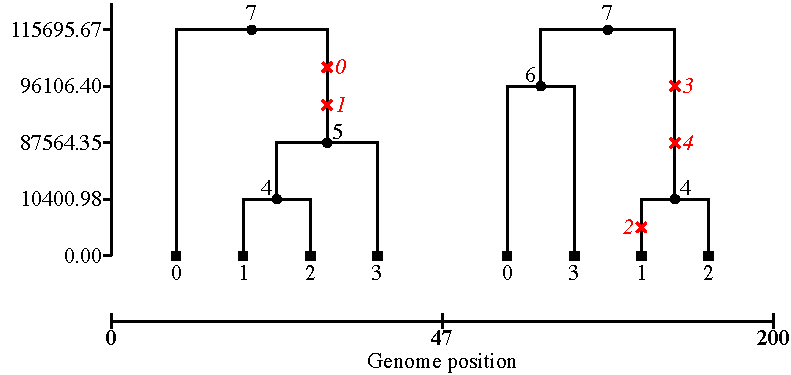
\includegraphics[width=\linewidth]{{union_example/example_ts.pdf}}
\caption{An example tree sequence.}\label{fig:example_ts}
\end{subfigure}
\begin{subfigure}[b]{.45\linewidth}
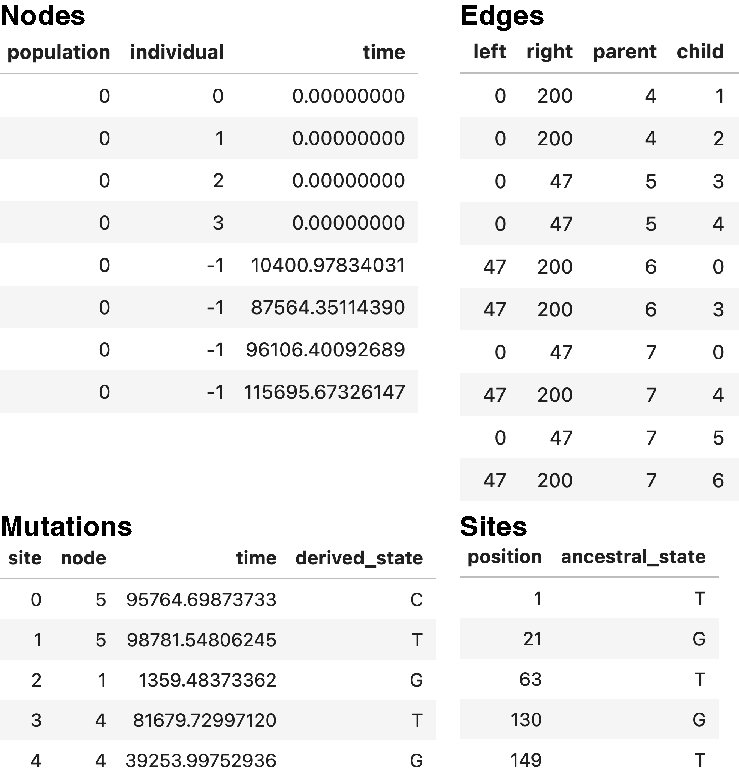
\includegraphics[width=\linewidth]{{union_example/tables.pdf}}
\caption{The underlying collection of tables.}\label{fig:table_collection}
\end{subfigure}
\caption[An example tree sequence and its tabular encoding]{
The relationship between four samples are depicted in a sequence of trees.
Note how because of shared ancestry,
mutations that are common to many of the samples need to be represented only once.
However, in a matrix of variant sites against samples, these mutations would be repeated unnecessarily.
}
\label{fig:example_ts_and_tc}
\end{figure}


After simulating two independent populations,
one might want to obtain the node-wise union of these two tree sequences (\eg for analyzing patterns of between population variation).
This is almost as simple as concatenating the Node, Edge, Site and Mutation tables.
However, nodes from the second tree sequence need to be re-enumerated, and this new numeric order needs to be propagated onto the other tables.
I simulated the history of two populations independently using \msprime \citep{kelleher_efficient_2016, baumdicker_efficient_2022} \plcref{fig:ts1,fig:ts2}.
Then, I used the union operation to merge the two tree sequences \plcref{fig:tsu}.
Lastly, I added the pre-split history to the merged tree sequence so that all samples coalesce back-in-time \plcref{fig:tsu_recap}.
See the code in Python to reproduce this analysis \plcref{code:union}.
By doing the simulation this way, we are able to run the simulation of each extant population in parallel.
In the case of large simulations (as we will see in \lcref{chapter:greatapes}),
this is essential so that we can distribute the memory usage over different computer nodes.

\begin{lstlisting}[language=Python, caption={Python code to union two independently simulated populations using \msprime and \tskit.}, label=code:union, breaklines=true]
import msprime
import numpy as np
import tskit

# First, we build an msprime.Demography object with our two-population history that splits 100,000 units of time ago
demography = msprime.Demography()
demography.add_population(name=``A'', initial_size=10_000)
demography.add_population(name=``B'', initial_size=100)
demography.add_population(name=``C'', initial_size=100_000)
demography.add_population_split(time=100_000, derived=[``A'', ``B''], ancestral=``C'')

# Now, we can simulate the histories of the two extant populations independently
ts1 = msprime.sim_ancestry(samples={``A'':4}, ploidy=1, demography=demography, sequence_length=50, recombination_rate=1e-6, random_seed=123)
ts2 = msprime.sim_ancestry(samples={``B'':4}, ploidy=1, demography=demography, sequence_length=50, recombination_rate=1e-6, random_seed=1)

# Then, we can union these two tree sequences.
# Note that because the two populations do not share any history,
# we specify a `node_mapping' in which none of the nodes in `ts2' have an equivalent in `ts1'.
tsu = ts1.union(ts2, node_mapping=np.full(ts2.num_nodes, tskit.NULL), add_populations=False)

# Finally, we can add the pre-split history to the union'ed tree sequence with msprime.sim_ancestry.
tsu_recap = msprime.sim_ancestry(initial_state = tsu, demography=demography, random_seed=3)
\end{lstlisting}

\begin{figure}
\centering
\begin{minipage}{0.45\textwidth}%
\begin{subfigure}[b]{\linewidth}
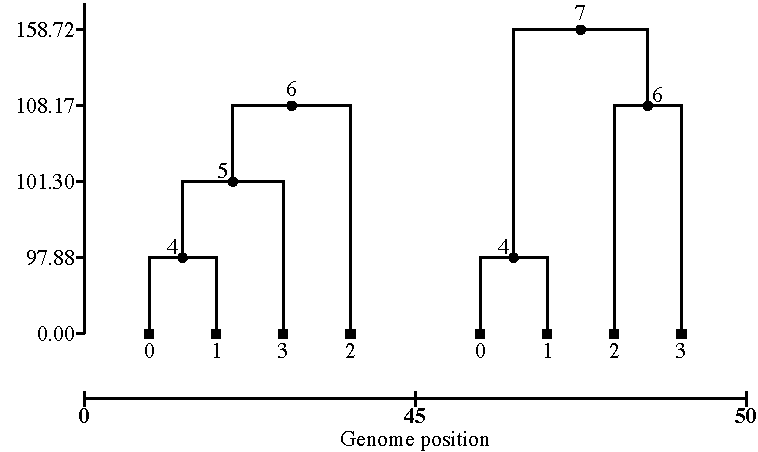
\includegraphics[width=\linewidth]{union_example/ts2.pdf}
\caption{Tree sequence of population 1.}\label{fig:ts1}
\end{subfigure}
\end{minipage}
\begin{minipage}{0.45\textwidth}%
\begin{subfigure}[b]{\linewidth}
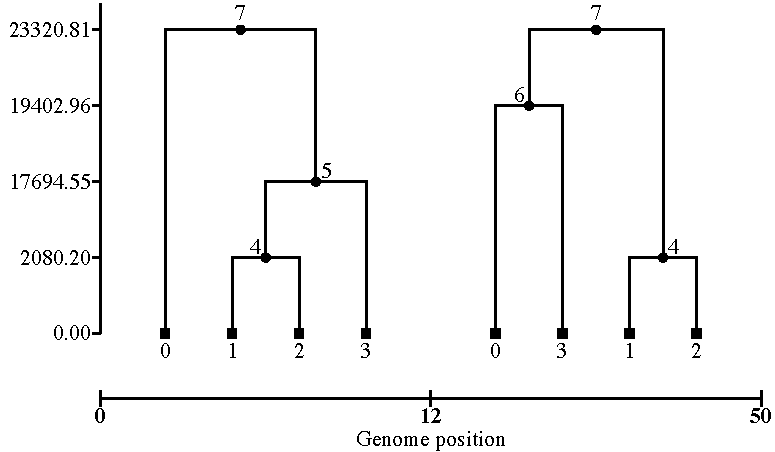
\includegraphics[width=\linewidth]{union_example/ts1.pdf}
\caption{Tree sequence of population 2.}\label{fig:ts2}
\end{subfigure}
\end{minipage}

\begin{subfigure}[b]{.9\textwidth}
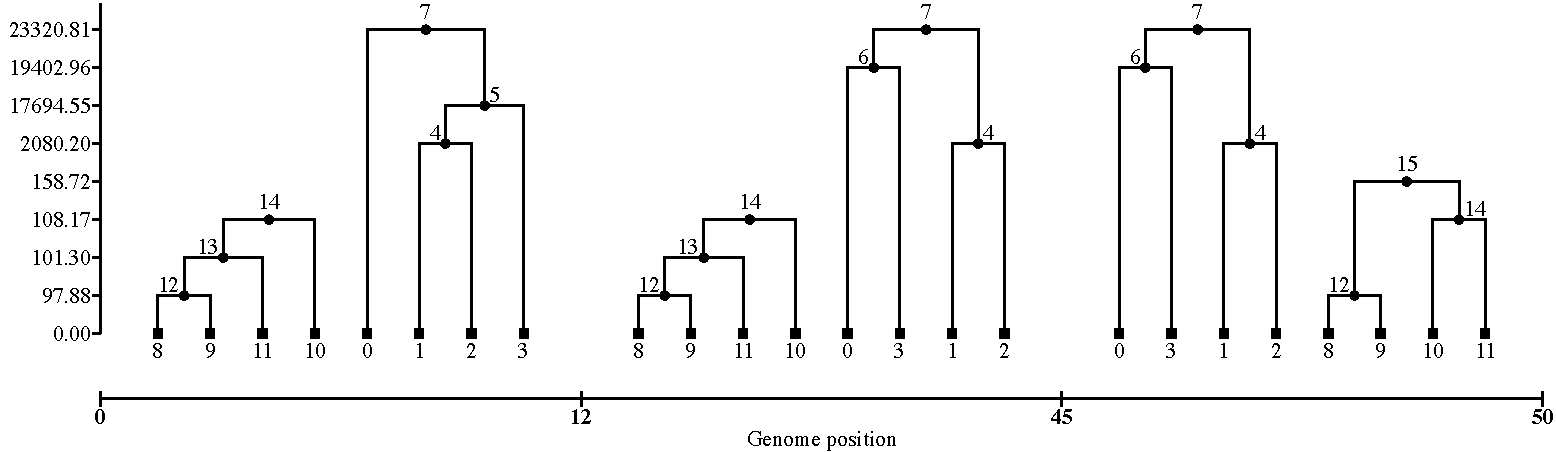
\includegraphics[width=\linewidth]{union_example/tsu.pdf}
\caption{Union of tree sequences 1 and 2.}\label{fig:tsu}
\end{subfigure}

\begin{subfigure}[b]{0.9\textwidth}
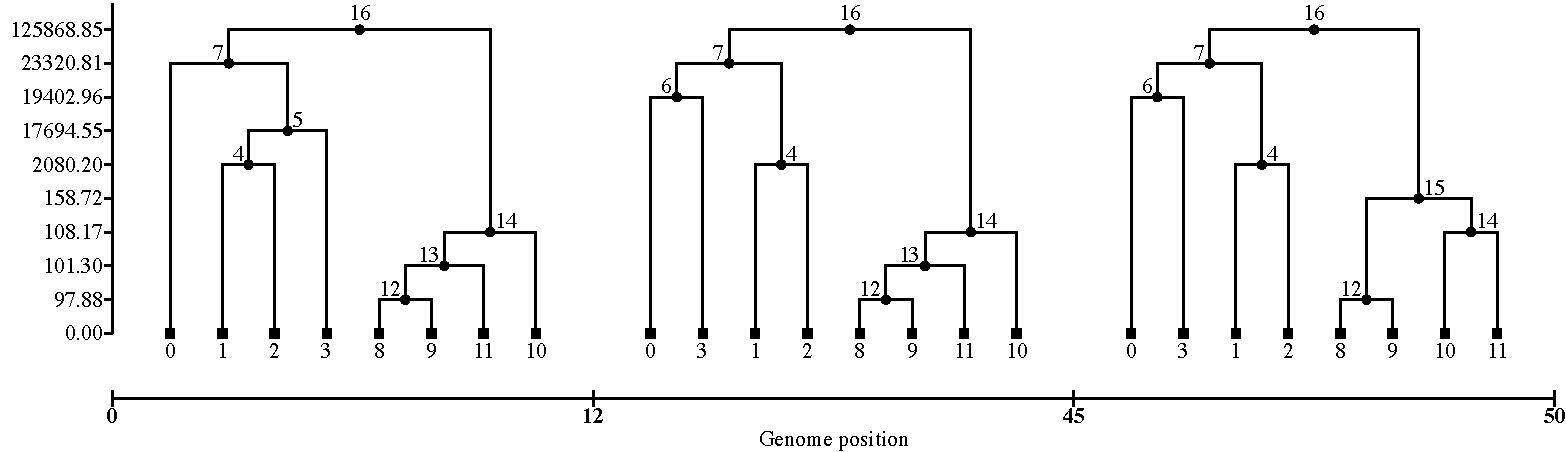
\includegraphics[width=\linewidth]{union_example/tsu_recap.pdf}
\caption{Adding the pre-split history to the union.}\label{fig:tsu_recap}
\end{subfigure}

\caption[The union operation for tree sequences]{The union operation for tree sequences.
(a) and (b) show the tree sequences for two independently simulated populations.
(c) depicts the union of these tree sequences.
(d) shows the merged tree sequences with added history for the ancestral population.}
\label{fig:union_op}
\end{figure}

A trickier use case for the node-wise union operation is when there are two tree sequences which share part of their histories.
That is, imagine you simulate the ancestor population of A and B, and then start two new independent simulations of A and B.
In this case, it is necessary to defined which portions are not shared between the two tree sequences,
so that the histories can be joined properly.
To define the non-shared portions, it is necessary to specify which nodes in one tree sequence are equivalent to those in the other.
Then, the portions that are not shared from one tree sequence are copied over onto the other.
New nodes are given a new numeric identifier which are propagated to the other tables.
Refer to \citet{rodrigues_vignette_2021} for a concrete example on how to union tree sequences with some shared history.

\section{Towards more realistic and reproducible simulations: Introducing models of selection to Stdpopsim}

Underlying adaptation to an environment, there can be a population genetic process called selective sweep.
As a new beneficial mutation increases in frequency due to positive selection it wipes out genetic variation surrounding the selected site \citep{smith_hitch-hiking_1974, kaplan_hitchhiking_1989}.
This footprint of the sweep can be used to infer instances of genetic adaptation.

Inferring selective sweeps has been a major area research in evolutionary genetics \citep{nielsen_estimation_2000, hernandez_classic_2011, garud_recent_2015, schrider_soft_2017, przeworski_signature_2002, enard_genome-wide_2014, williamson_evidence_2014}.
Our ability to detect selective sweeps depends on many parameters, such as the recombination rate, the time since fixation, and the demographic history.
The recombination rate determines the width of a selective signal (together with the strength of selection) \citep{kaplan_hitchhiking_1989}.
As time passes by, new mutations are accumulated restoring pre-sweep levels of genetic variation and erasing sweep signatures.
Demographic events can leave footprints similar to a selective sweep, confounding detection \citep{przeworski_signature_2002, jensen_distinguishing_2005}.
Conversely, sweep signatures can be erased by recent demographic events, such as bottlenecks.

Another process that can impact our ability to detect sweeps is background selection.
Background selection is the process whereby neutral genetic variation linked to deleterious mutations are lost \citep{charlesworth_effect_1993}, and the extent of this effect is also modulated by strength of selection and recombination rate.
Because of this relationship with recombination rate, background selection can confound the search for selective sweeps \citep{andolfatto_adaptive_2001}.
This process seems to be pervasive in multiple species; so much so that background selection may be considered a better null hypothesis in population genomic studies rather than neutrality \citep{comeron_background_2017}.

With a more realistic spatial arrangement of constrained sites, background selection may be discernible from a selective sweep \citep{schrider_background_2020}.
Previous studies that found background selection can confound sweep calling assumed that the region constrained by selection is flanked by large streches of neutral sites,
but the locations of exons and other constrained elements are usually scattered throughout the chromosome.

To better understand the role of positive selection in shaping genetic variation across the genome,
it is necessary to better delineate how different processes impact our ability to detect selective sweeps.
I present  below our efforts to include models of natural selection to Stdpopsim, our community-driven library of evolutionary models.
We included the ability to easily simulate background selection and selective sweeps using previously published distribution of fitness effects (DFEs).
We demonstrate this new feature by analyzing how power to detect selective sweeps varies over a realistic looking human chromosome, with recombination rate variation and a map of constraint taken from human annotations.

\subsection{Adding selection to simulations using Stdpopsim}

There are two main ways of adding selection to a simulation in stdpopsim: (i) it is possible to specify a distribution of fitness effects (DFE) for new mutations that can occur across the genome or over some pre-specified regions; and (ii) we can introduce and track a single mutation to a population, as one would need to study selective sweeps.
Beyond the machinery to actually perform these two kinds of simulations, we now added to Stdpopsim a library of previously published distributions of fitness effects and genomic annotations (\eg exon and intron coordinates) which can be used to build realistic models with selection.
See our Tutorial for more details on how to implement models with selection in stdpopsim: \url{https://popsim-consortium.github.io/stdpopsim-docs/stable/tutorial.html#incorporating-selection}.

\subsection{Analysis of power to detect sweeps along realistic chromosomes}

To demonstrate the utility of stdpopsim, we produced maps of power to detect sweeps along a realistic chromosome.
We ran simulations of human chromosome 1 using the three population out-of-Africa model (identified as OutOfAfrica\_3G09 in the stdpopsim library; \cite{gutenkunst_inferring_2009}) and the genetic map estimated in \citet{frazer_second_2007} (HapMapII\_GRCh38).
For computational efficiency, we simulated a 5Mb region flanking 100 evenly distributed points along the chromosome 1.
We had four classes of simulations: (i) neutral (with the specified demography and genetic map), (ii) background selection, in which we applied the DFE estimated in \citet{kim_inference_2017} (Gamma\_K17) to exon annotations (taken from Ensembl; ensembl\_havana\_104\_exons), (iii) sweep, in which we simulated a hard selective sweep at the center of the focal point (with selection coefficient of $s=0.03$; we only kept simulations for which the beneficial mutation reached at least 95\% frequency), and (iv) sweep with background selection, in which we simulated the hard sweep as described with the addition of constraint in exonic regions (same as for \emph{ii}).
To prevent distortions at the edges of the simulated 5Mb regions, we added a buffer of 2.5cM flanking the region.
In total, we produced 200 replicates for each class at each poisition, totalling 80,000 simulations.
We rescaled the simulations to reduce computational cost by simulating smaller populations (factor of 2) while increasing times, mutation and recombination rates, and selection coefficients by the same amount (see \cite{uricchio_robust_2014} and \cite{adrion_community-maintained_2020} for more details).
